\documentclass[residuals.tex]{subfiles}
\begin{document}
\Large	
\section{Simple Linear Regression}	
In simple linear regression, we predict values on one variable from the values of a second variable. 

\begin{itemize}
\item The variable we are predicting is called the \textbf{\textit{dependent variable}} (or response variable) and is referred to as Y. 

\item The variable we are basing our predictions on is called the \textbf{i\textit{ndependent variable}} (or predictor variable) and is referred to as X.
\end{itemize} \textit{
\noindent Remark: When there is only one predictor variable, the prediction method is called simple regression. Linear regression can have more than one predictor variable, i.e. Multiple Linear Regression.}
\newpage

\bigskip 
\noindent In simple linear regression, the predicted values of Y when plotted as a function of X form a straight line on the scatter plot. This line is known as the \textbf{\textit{regression line}}. 

\begin{figure}[h!]
\centering
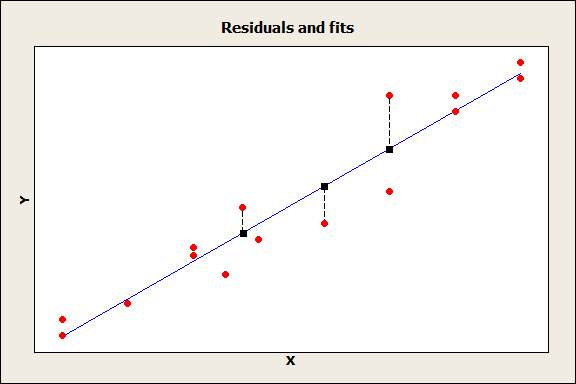
\includegraphics[width=0.9\linewidth]{resids1}
\caption{}
\label{fig:resids1}
\end{figure}

\begin{itemize}
\item Suppose we construct our model using $n$ observed values of the response variable $y_1, y_2, \ldots y_i \ldots y_n$

\item For the original data set, there is a predicted value of each case of $Y$ that corresponds to an observed value of $Y$. 

\item The difference between an observed value of the dependent variable ($y_i$) and the corresponding predicted value ($\hat{y}$) is called the residual ($e_i$). Each data point from the data set has one residual.

\item Simply put, the values of the residuals are derived as follows: 
\[\mbox{Residual = Observed value - Predicted value}\]
\[e_i = y_i - \hat{y_i} \]
\item For three cases in the graphic above, the observed value (red dot) is linked to its corresponding predicted value (black dot) on the regression line (blue line).
The difference (i.e. residual) is depicted using a dashed line. The magnitude of these residuals is of interest.
\item The second of the three residuals will have a negative value.
\item \textbf{\textit{Ordinary Least Squares}} is a method of fitting a model, such that the total residual values are minimised.


\item Important theoretical assumption underlying the OLS model: the sum of the residuals should equal to zero. 

{
\Large
\[\sum e_i = 0\]
}
\item An extension of this is that the expected value of the residuals is 0. 
$\mathrm{E}(e) = 0$
\item Another Important Theoretical Assumption - The residuals are normally distributed. (more on that later)
\end{itemize}

\subsection{Residual Plots}
A residual plot is a graph that shows the residuals on the vertical axis and the independent variable on the horizontal axis. If the points in a residual plot are randomly dispersed around the horizontal axis, a linear regression model is appropriate for the data; otherwise, a non-linear model is more appropriate.

\newpage
\subsection*{Summary of Important Terms}
Some important terms in model diagnostics, essentially a plan for this talk.
\begin{description}
	\item[Residual: ] The difference between the predicted value (based on the regression equation) and the actual, observed value.
	\item[Outlier:]  In linear regression, an outlier is an observation with large residual.  In other words, it is an observation whose dependent-variable value is unusual given its value on the predictor variables.  An outlier may indicate a sample peculiarity or may indicate a data entry error or other problem. 
	\item[Leverage:]  An observation with an extreme value on a predictor variable is a point with high leverage.  Leverage is a measure of how far an independent variable deviates from its mean.  High leverage points can have a great amount of effect on the estimate of regression coefficients. 
	\item[Influence:]  An observation is said to be influential if removing the observation substantially changes the estimate of the regression coefficients.  Influence can be thought of as the product of leverage and outlierness.  
	\item[Cook's distance (or Cook's D):] A measure that combines the information of leverage and residual of the observation.  
\end{description}

\subsection*{MultiCollinearity}

An importan aspect in model diagnostics is checking for multicollinearity. We are not going to cover this in this talk - but rather include in n a talk about variable selection procedure.
\newpage
\end{document}

